\documentclass[aspectratio=169]{beamer}

% Theme and color scheme
\usetheme{Madrid}
% Packages
\usepackage{amsfonts,amssymb}
\usepackage{graphicx}
\usepackage{tikz}
\usepackage{fontawesome5}
\usepackage{xcolor} 
\usepackage{booktabs}
\usepackage{subcaption}

% Custom colors - Bordeaux theme
\definecolor{primarycolor}{RGB}{128,0,32}      % Bordeaux rot
\definecolor{secondarycolor}{RGB}{165,42,42}   % Helleres Bordeaux
\definecolor{accentcolor}{RGB}{220,20,60}      % Crimson als Akzent
\definecolor{darkbordeaux}{RGB}{90,0,22}       % Dunkleres Bordeaux

% Set colors
\setbeamercolor{structure}{fg=darkbordeaux}
\setbeamercolor{frametitle}{bg=darkbordeaux,fg=white}
\setbeamercolor{title}{fg=white}
\setbeamercolor{palette primary}{use=structure,fg=white,bg=darkbordeaux}
\setbeamercolor{palette secondary}{use=structure,fg=white,bg=darkbordeaux}
\setbeamercolor{palette tertiary}{use=structure,fg=white,bg=darkbordeaux}
\setbeamercolor{normal text}{fg=darkbordeaux}
\setbeamercolor{item}{fg=darkbordeaux}
\setbeamercolor{itemize item}{fg=darkbordeaux}
\setbeamercolor{itemize subitem}{fg=darkbordeaux}
\setbeamercolor{enumerate item}{fg=darkbordeaux}
\setbeamercolor{section in toc}{fg=darkbordeaux}
\setbeamercolor{caption}{fg=darkbordeaux}

% Remove navigation symbols
\setbeamertemplate{navigation symbols}{}

% Empty footer
\setbeamertemplate{footline}{}

% Title page information
\title[Academic Presentation]{Lucas Hirschfeld}
\subtitle{Presentation for TIDE interview}
\institute[Uni Bonn]{
    Rheinische Friedrich-Wilhelms-Universität Bonn\\
    Department of Physical Chemistry}
\date{September 18, 2025}

\begin{document}

% Title slide
\begin{frame}
    \titlepage
\end{frame}

% About me section
\section{About Me}

\begin{frame}{Personal Information}
    \begin{columns}[c]
        \begin{column}{0.6\textwidth}
            \begin{itemize}
                \item \faUser\ Lucas Hirschfeld
                \item \faBirthdayCake\ Born August 14, 2000
                \item \faMapMarker*\ Bergfeldstraße 9, 53121 Bonn, Germany
                \item \faEnvelope\ hirschfeld@pc.uni-bonn.de
                \item \faGraduationCap\ M.Sc. Chemistry (expected 2025)
                \item \faGraduationCap\ B.Sc. Chemistry (2024)
            \end{itemize}
        \end{column}
        \begin{column}{0.4\textwidth}
            \begin{center}
                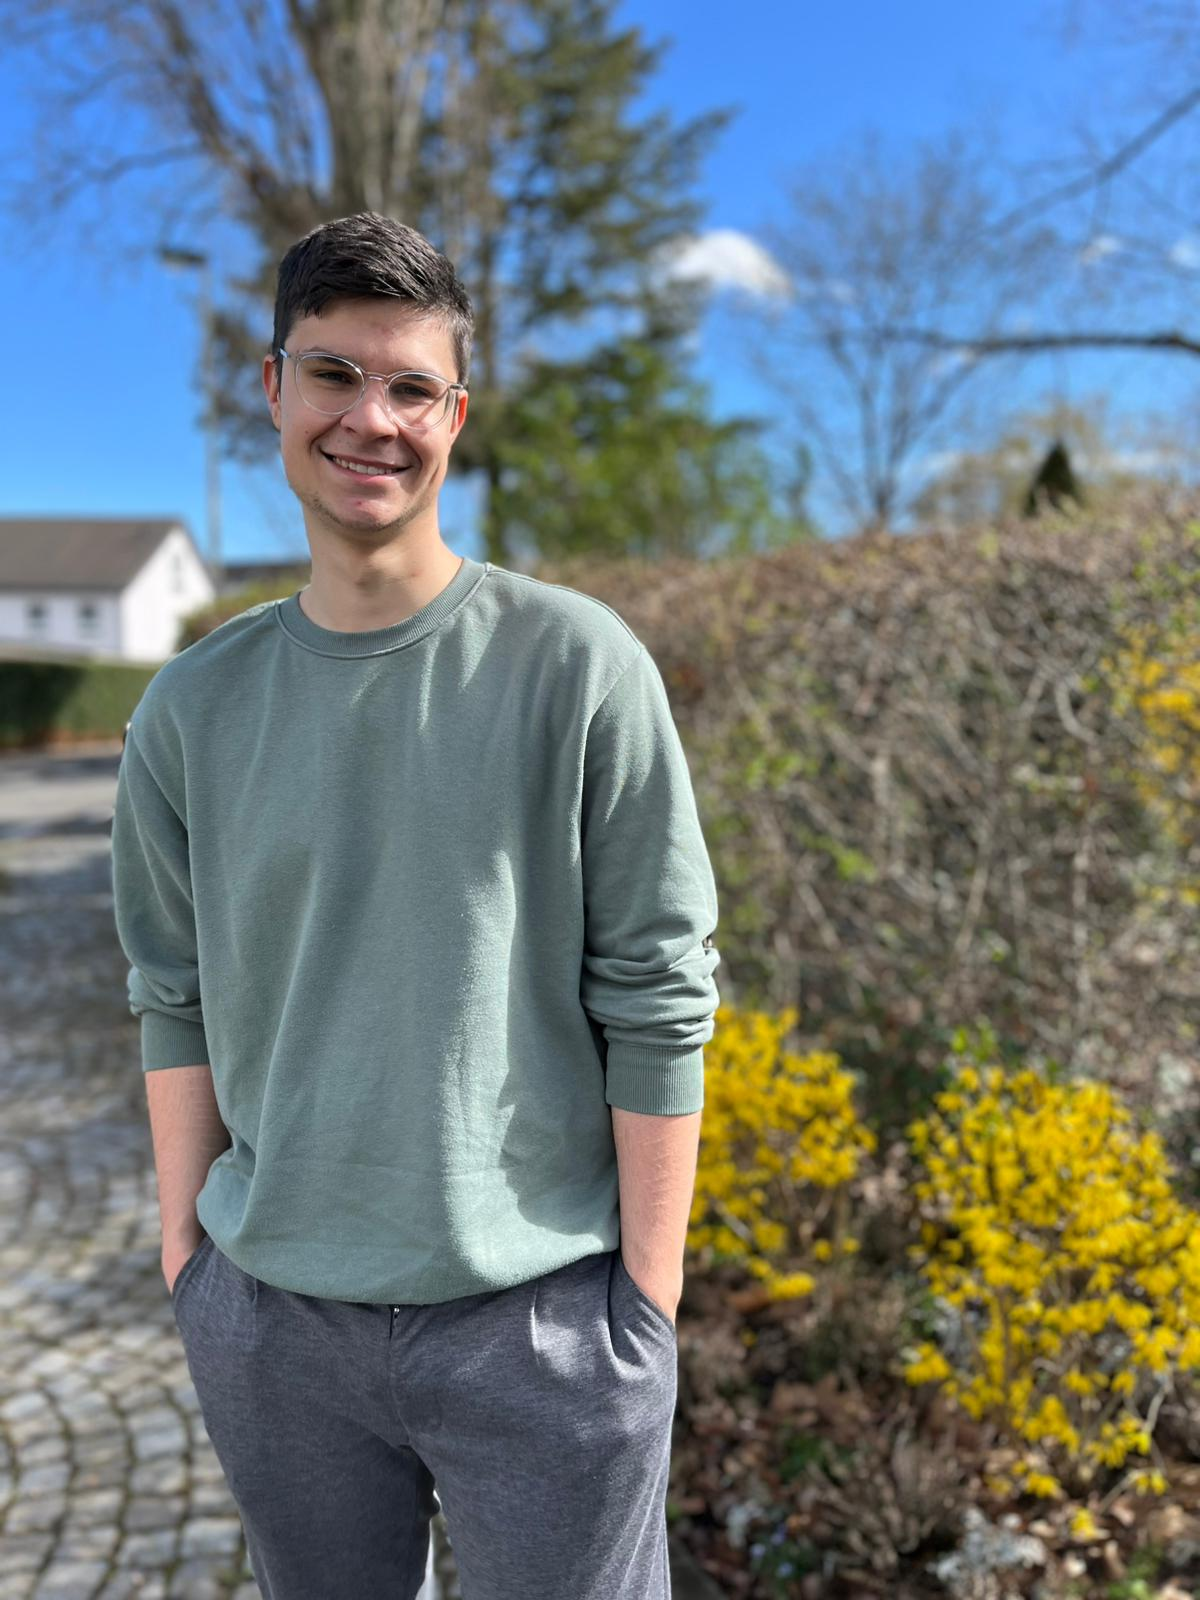
\includegraphics[width=0.7\textwidth]{images/me.jpeg}
            \end{center}
        \end{column}
    \end{columns}
\end{frame}

% Hobbies section
\begin{frame}{My Hobbies}
    \begin{columns}[c]
        \begin{column}{0.5\textwidth}
            \begin{center}
                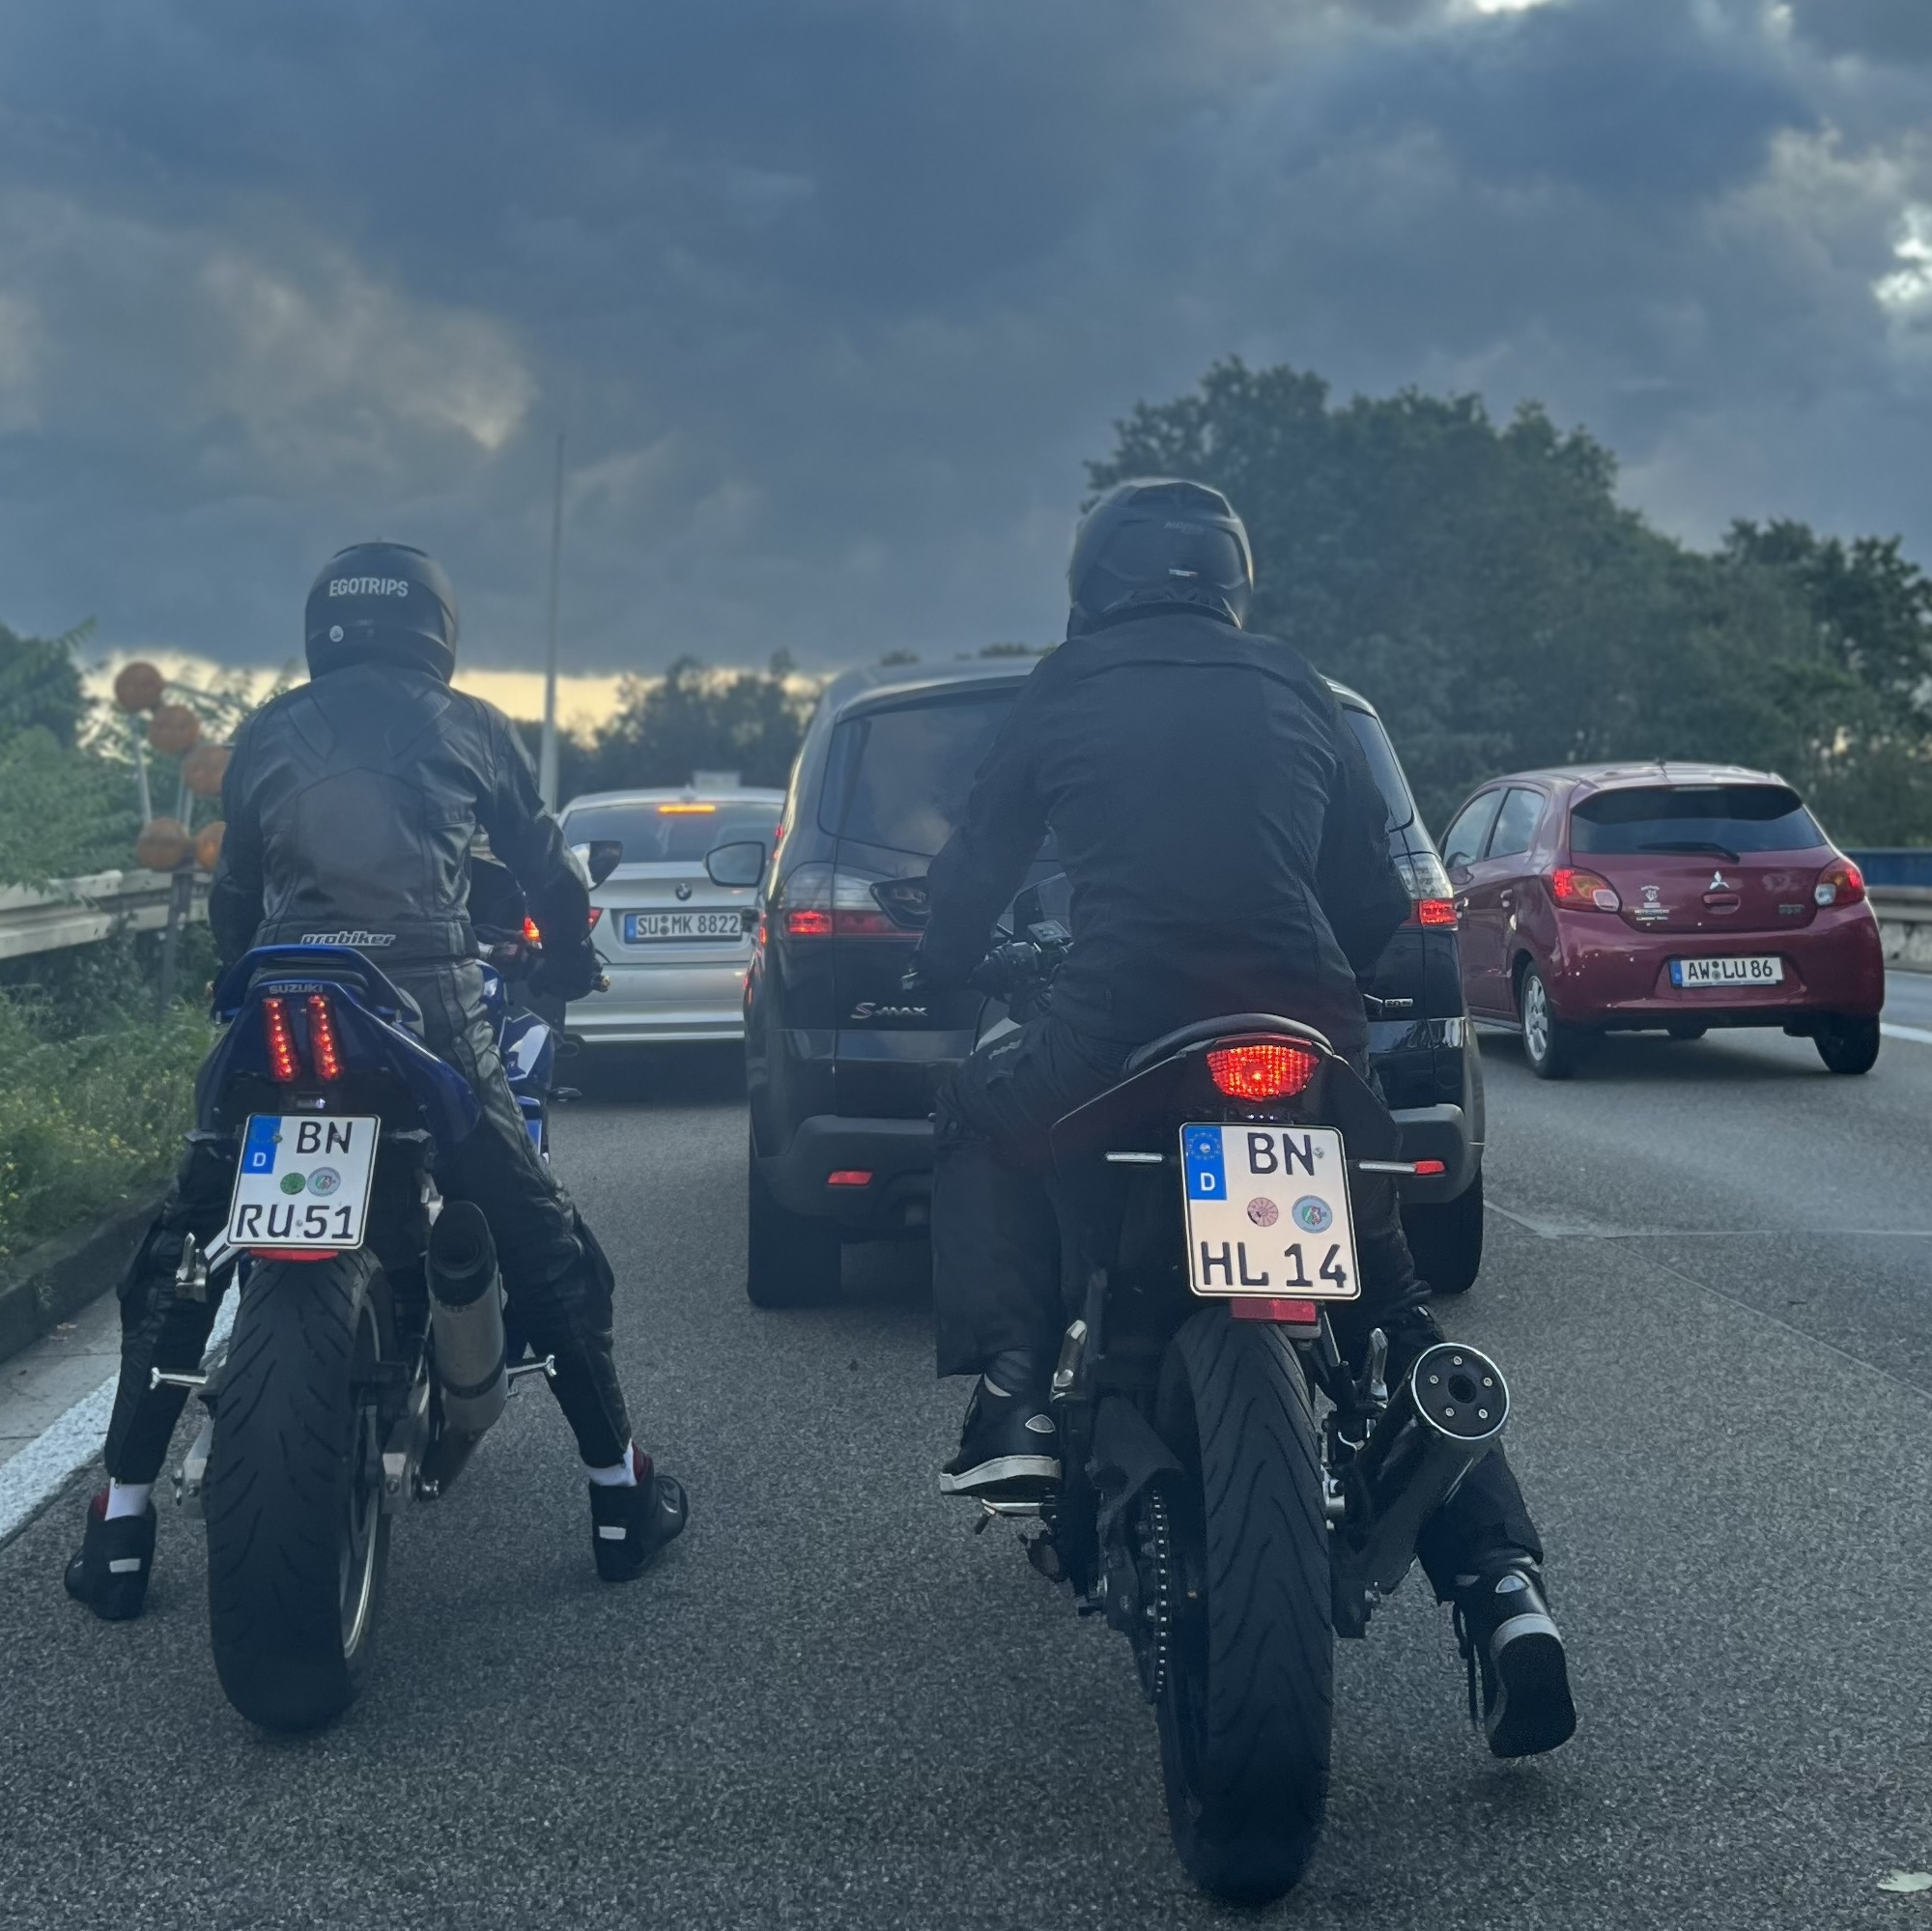
\includegraphics[width=0.8\textwidth]{images/motorcycle.jpeg}\\
                \small{Motorcycling}
            \end{center}
        \end{column}
        \begin{column}{0.5\textwidth}
            \begin{center}
                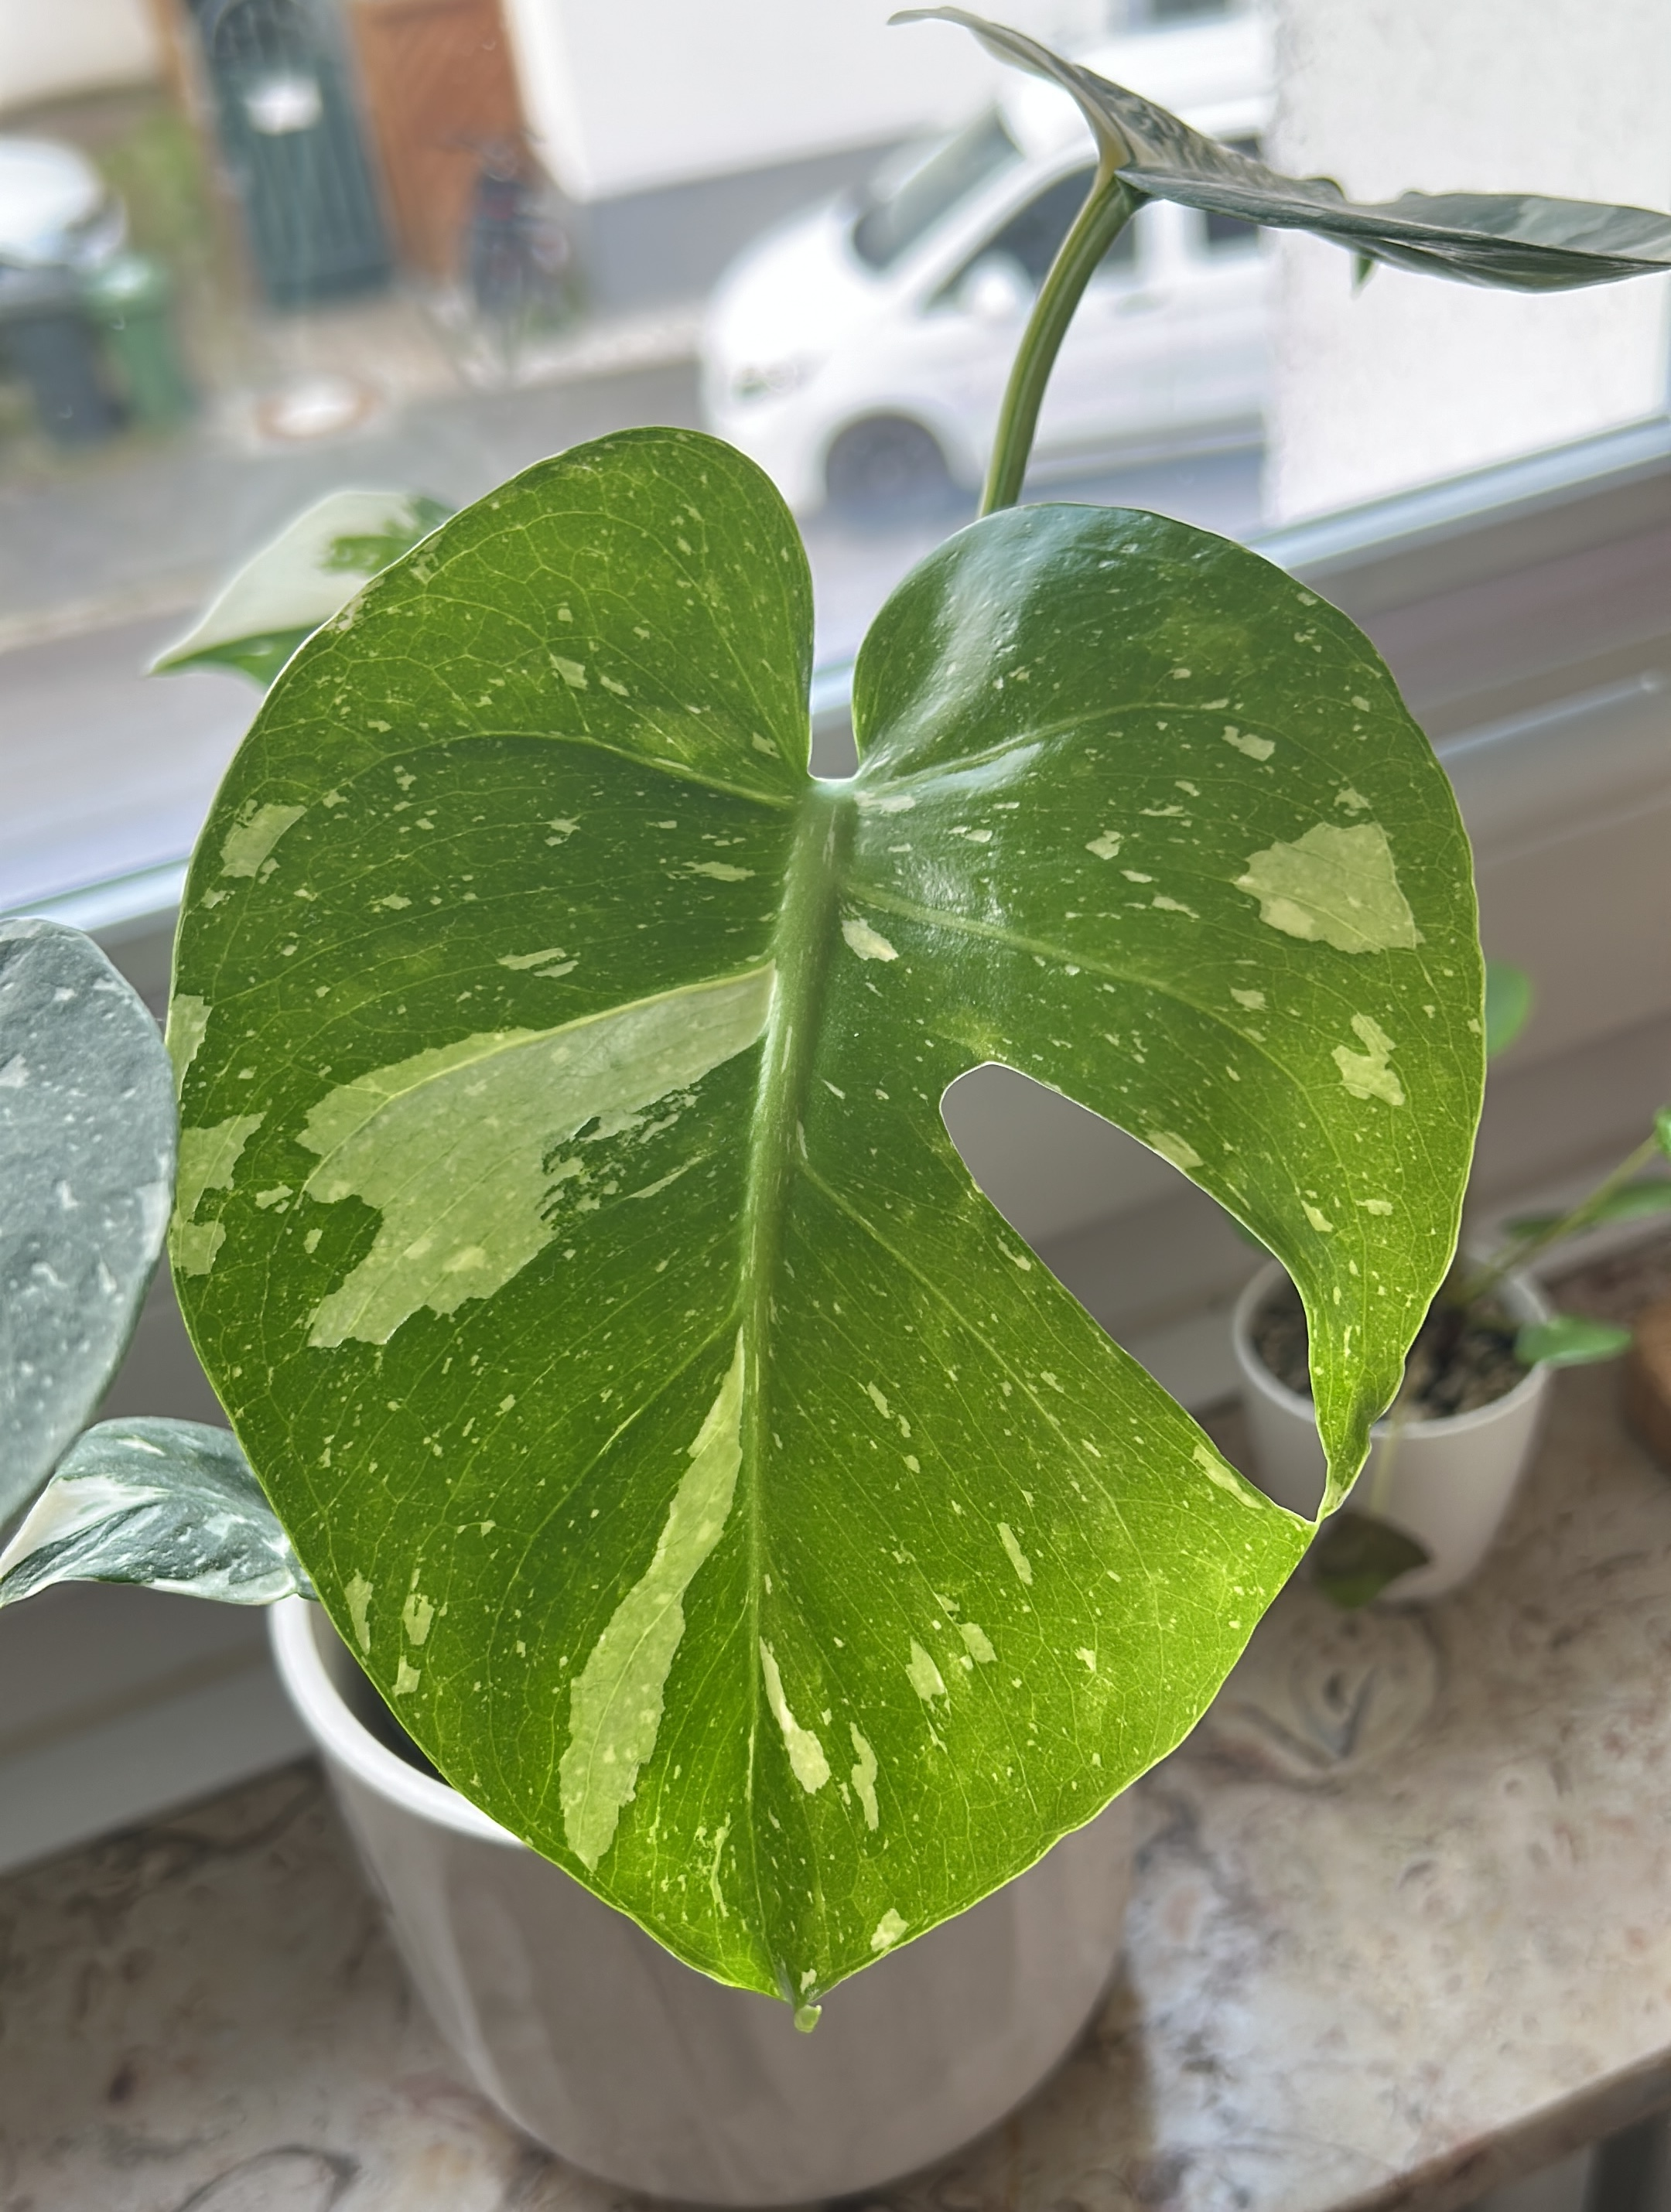
\includegraphics[width=0.65\textwidth]{images/plants.jpeg}\\
                \small{Exotic Plants}
            \end{center}
        \end{column}
    \end{columns}
\end{frame}

% Research Interests
\section{Research and Academic Work}

\begin{frame}{Bachelor Thesis Research}
    \begin{center}
        \setbeamercolor{mybox}{bg=darkbordeaux, fg=white}
        \begin{beamercolorbox}[wd=\textwidth, sep=0em, center, rounded=true]{mybox}
            \textbf{Thermische Desorptionsspektroskopie von Merocyaninen auf Ag(100)}
        \end{beamercolorbox}
    \end{center}
    
    \vspace{0em}
    
    \begin{columns}[c]
        \begin{column}{0.5\textwidth}
            \begin{center}
                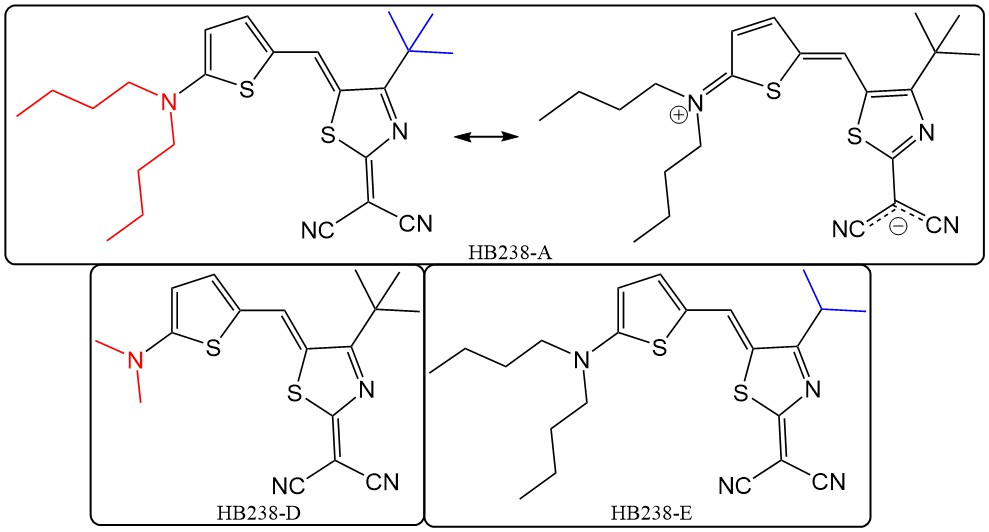
\includegraphics[width=\textwidth]{images/HB238_A-D-E.jpg}
                \\ \small{Structures of studied molecules}
            \end{center}
        \end{column}
        \begin{column}{0.5\textwidth}
            \begin{center}
                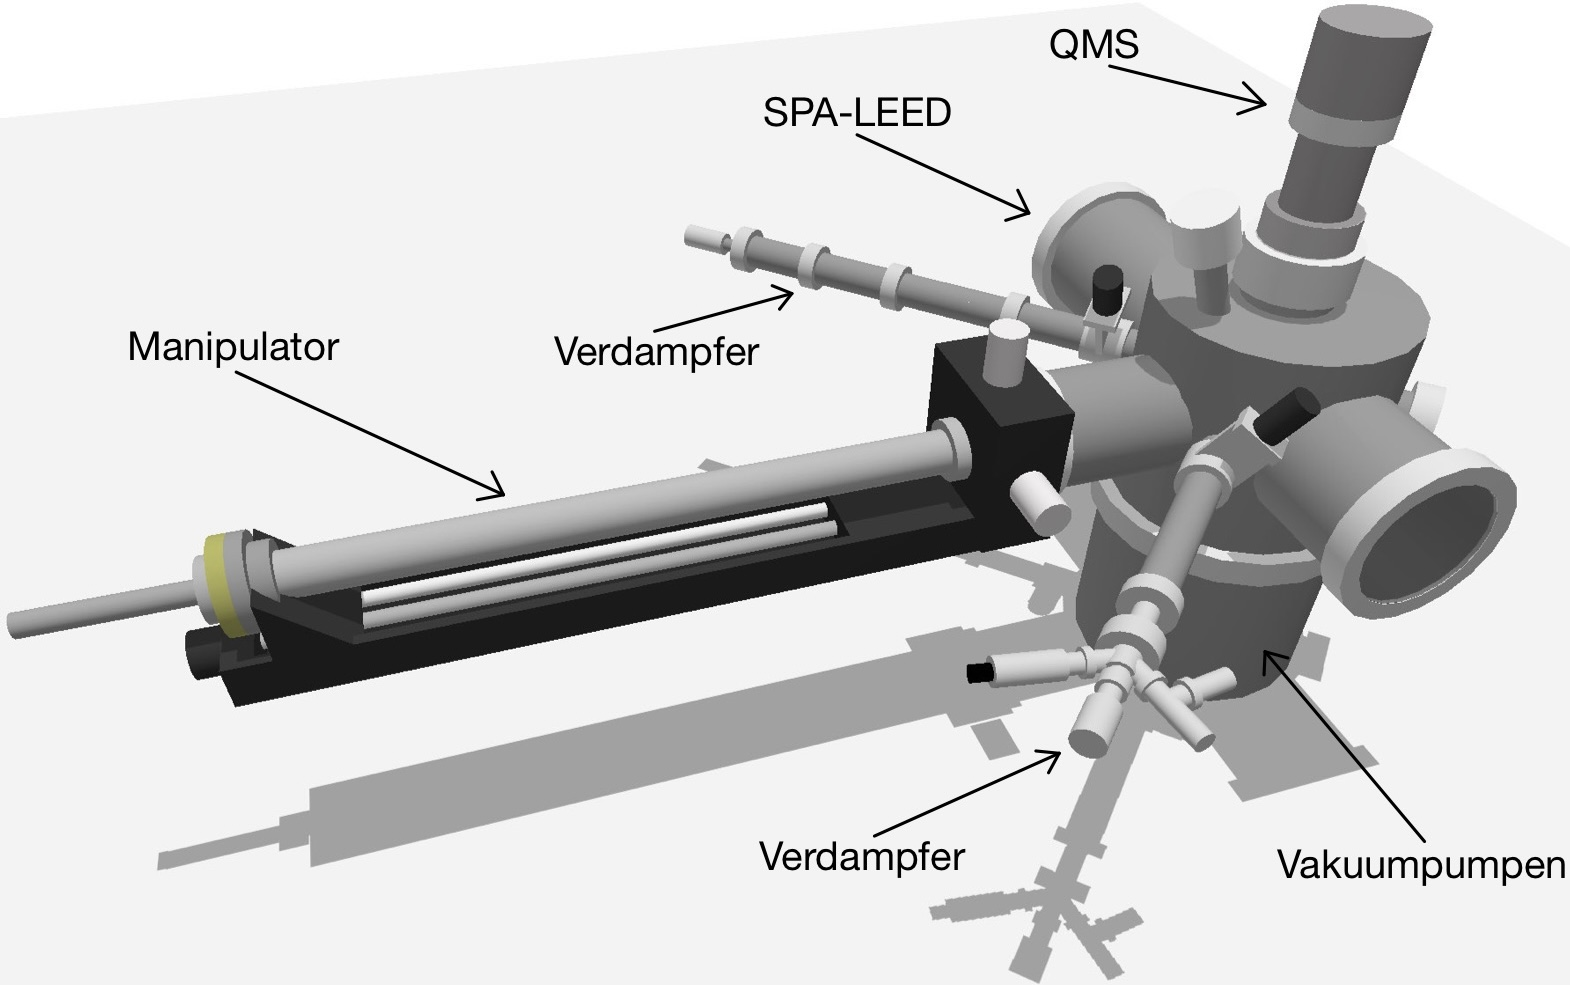
\includegraphics[width=\textwidth]{images/Aufbau.jpeg}%
                \\ \small{Research Setup}
            \end{center}
        \end{column}
    \end{columns}
\end{frame}

\begin{frame}{Bachelor Thesis Results}
    
    \begin{columns}[c]
        \begin{column}{0.5\textwidth}
            \begin{center}
                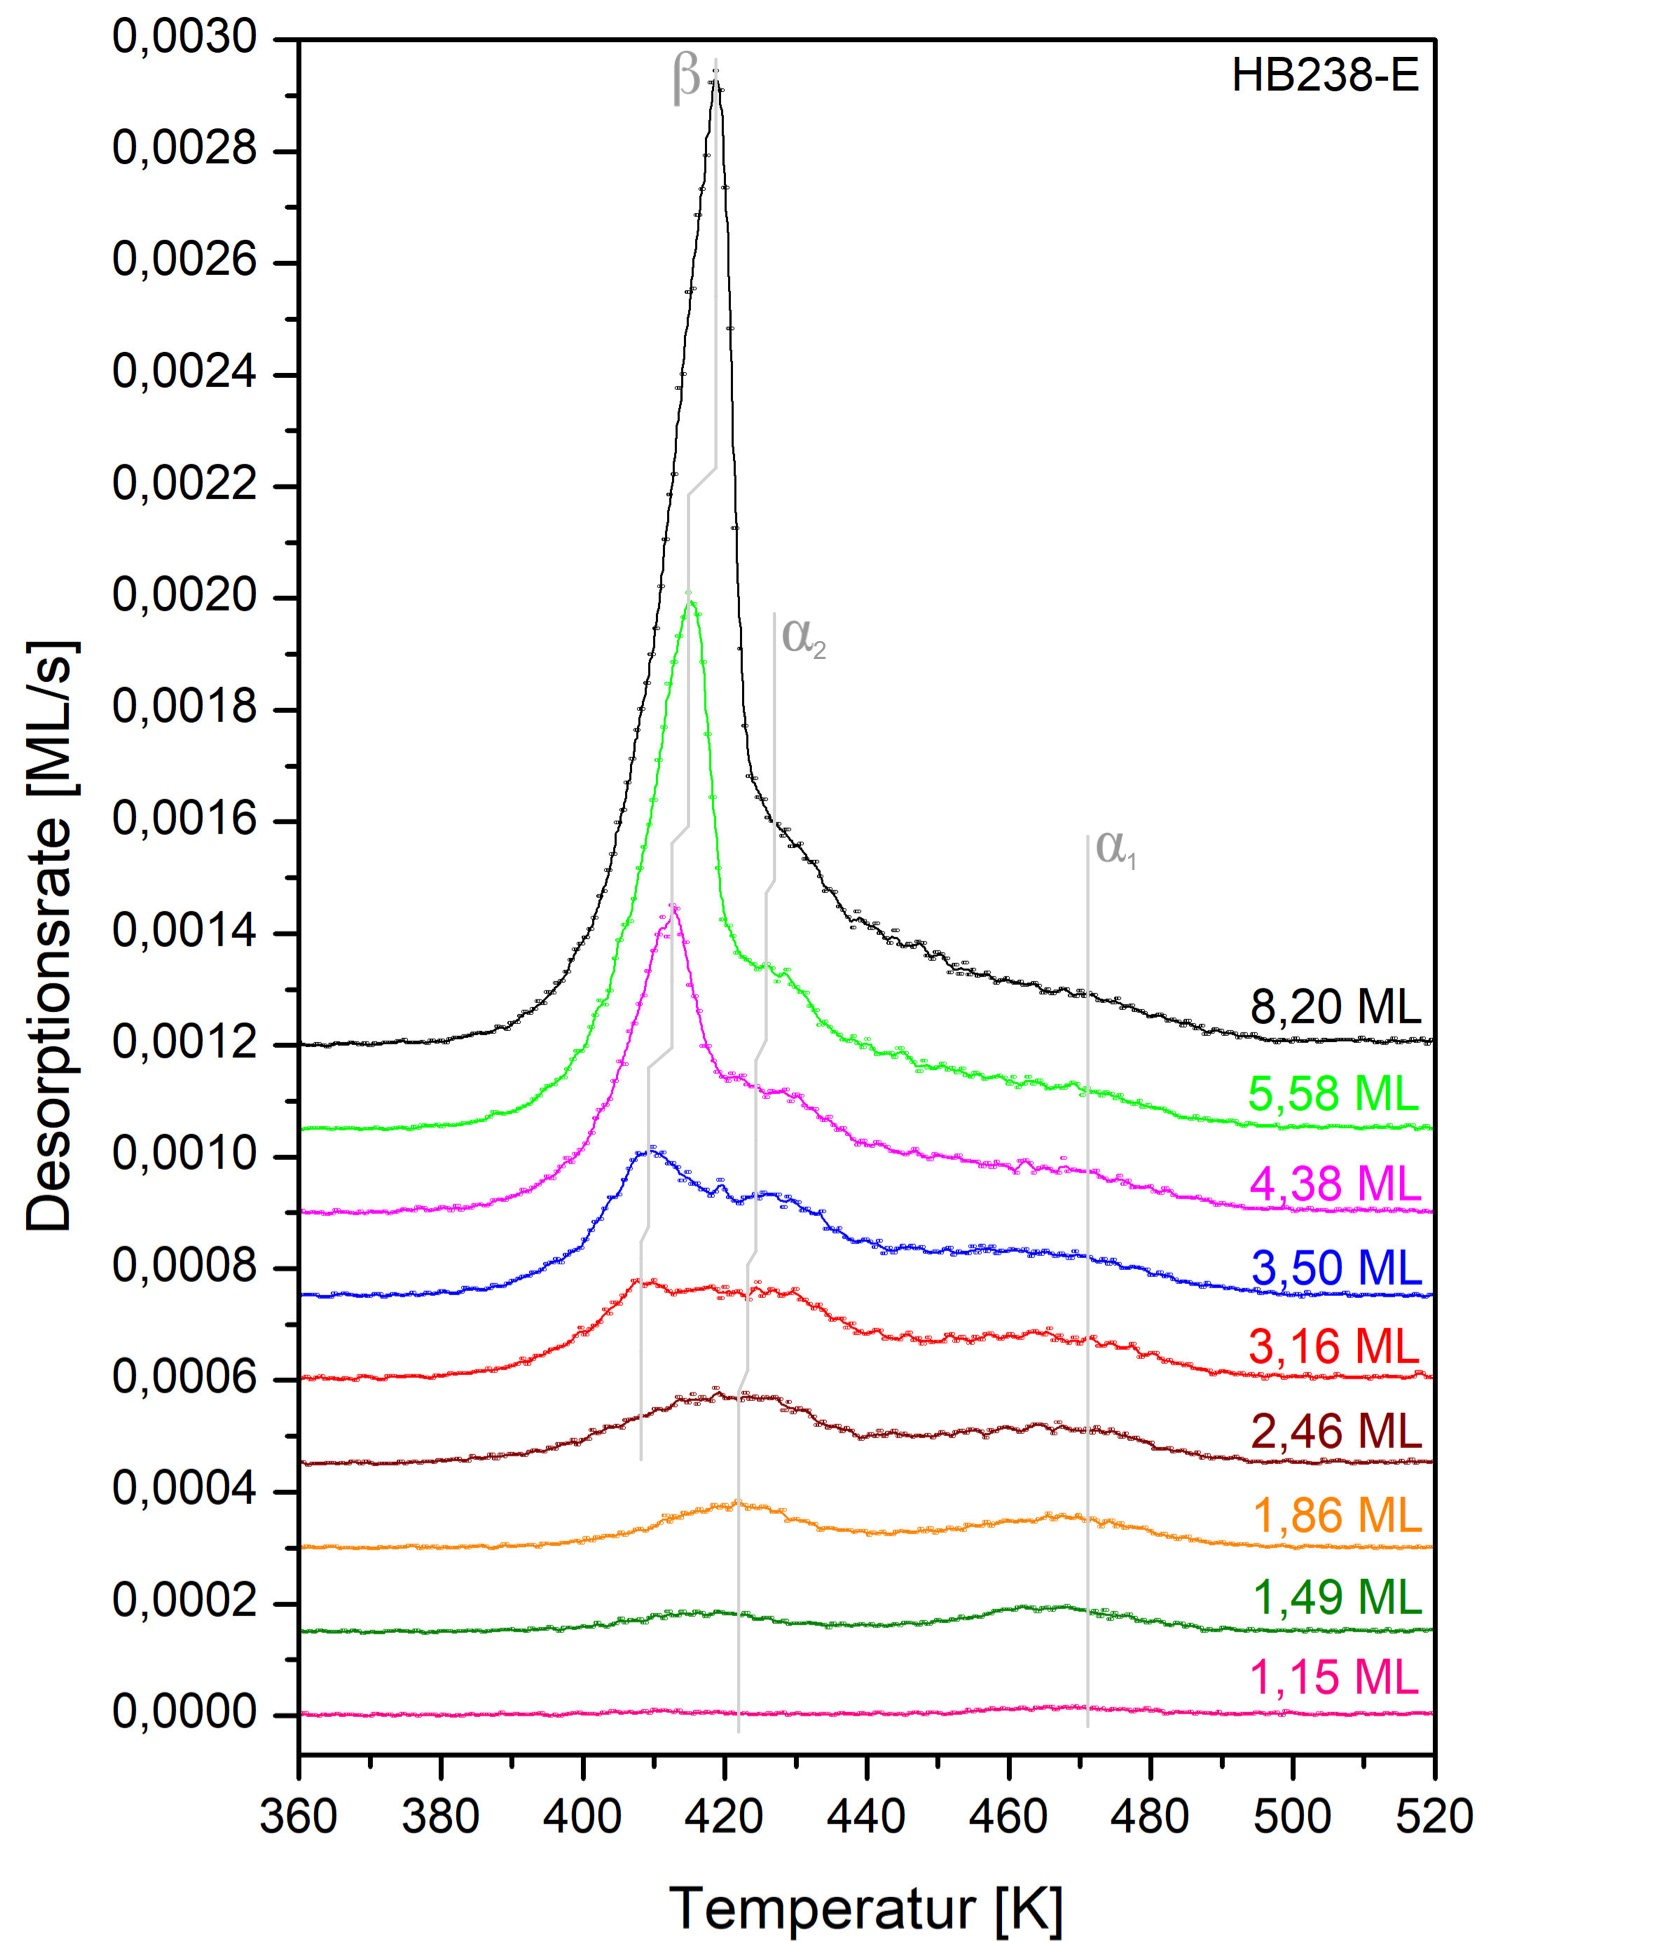
\includegraphics[width=0.75\textwidth]{images/TPD-HB238E.png}%
                \\ \small{TPD spectra of HB238-E on Ag(100)}
            \end{center}
        \end{column}
        \begin{column}{0.5\textwidth}
            \begin{center}
                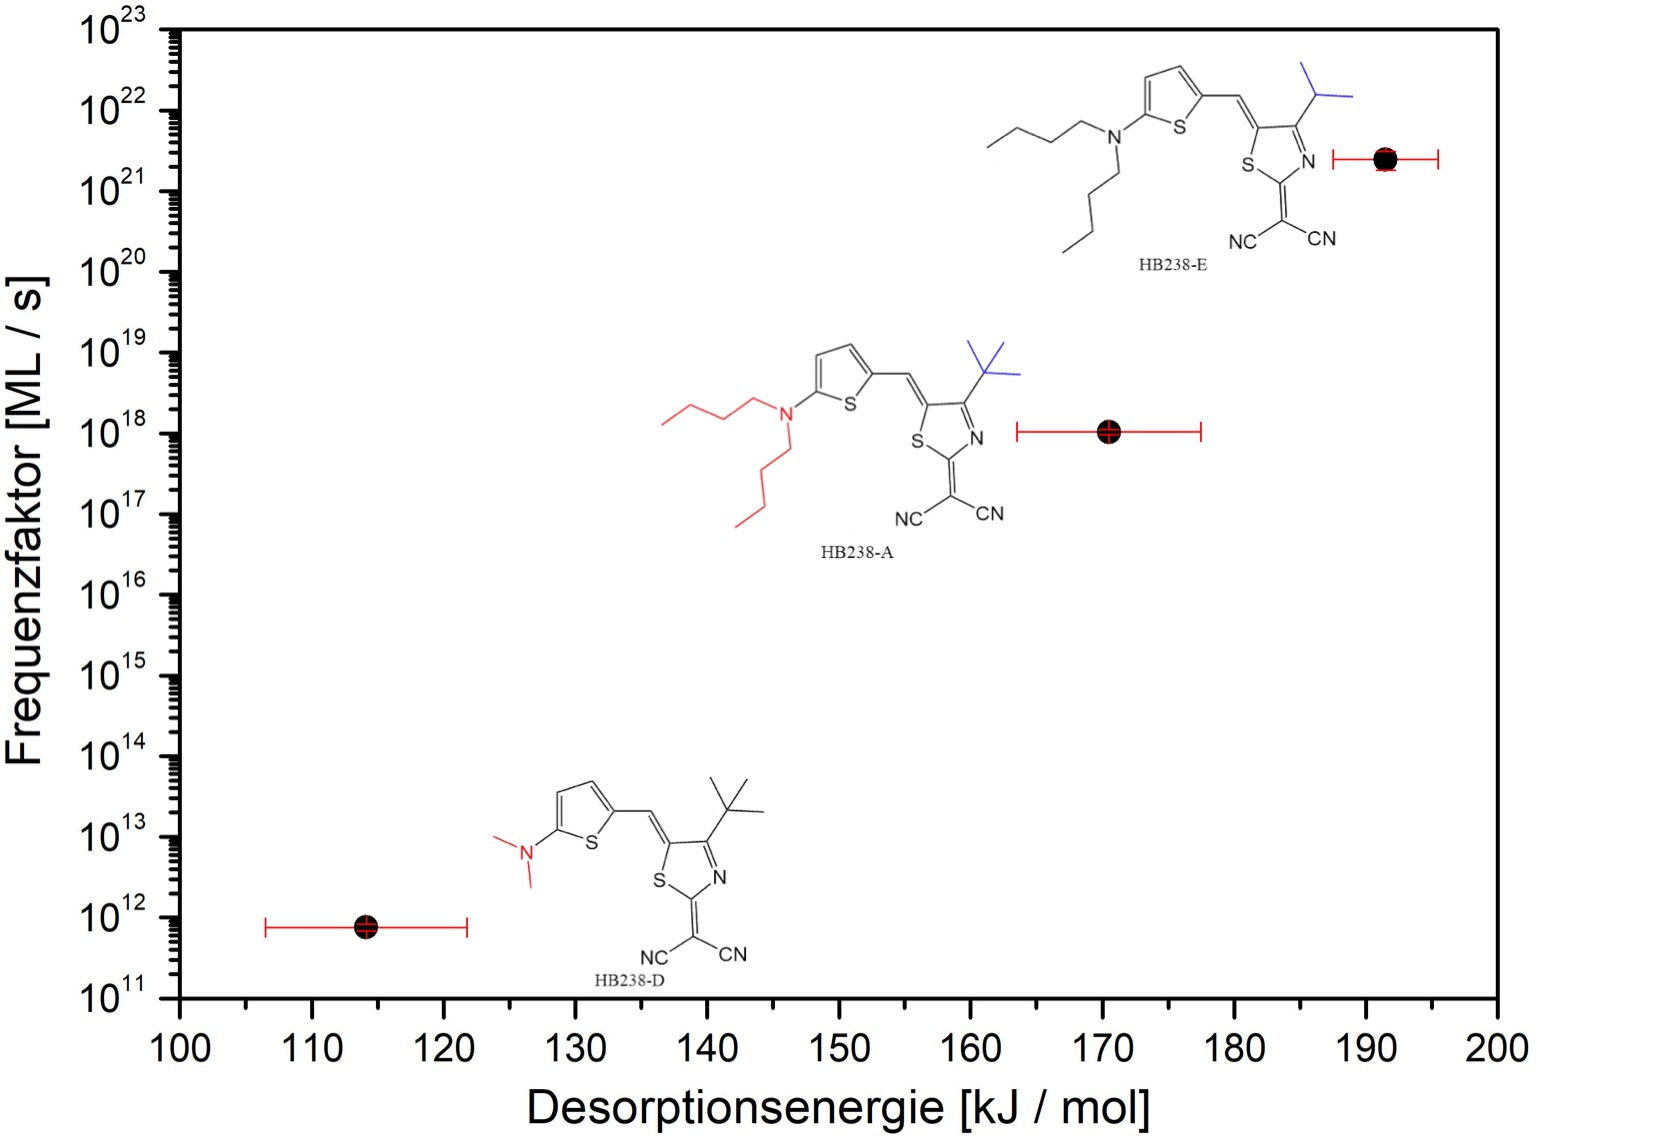
\includegraphics[width=1.1\textwidth]{images/E-gg-v.jpeg}%
                \\ \small{Desorption energy vs. pre-exponential factor}
            \end{center}
        \end{column}
    \end{columns}
\end{frame}


\begin{frame}{Current Master Studies}

    \vspace{0em}
    \begin{center}
        \setbeamercolor{mybox}{bg=darkbordeaux, fg=white}
        \begin{beamercolorbox}[wd=\textwidth, sep=0em, center, rounded=true]{mybox}
            \large{XPS \& NIXSW of Quinacridone on the Ag(100) surface}
        \end{beamercolorbox}
    \end{center}

    \vspace{-1em}
    \begin{columns}[c]
        \begin{column}{0.5\textwidth}
            \begin{center}
                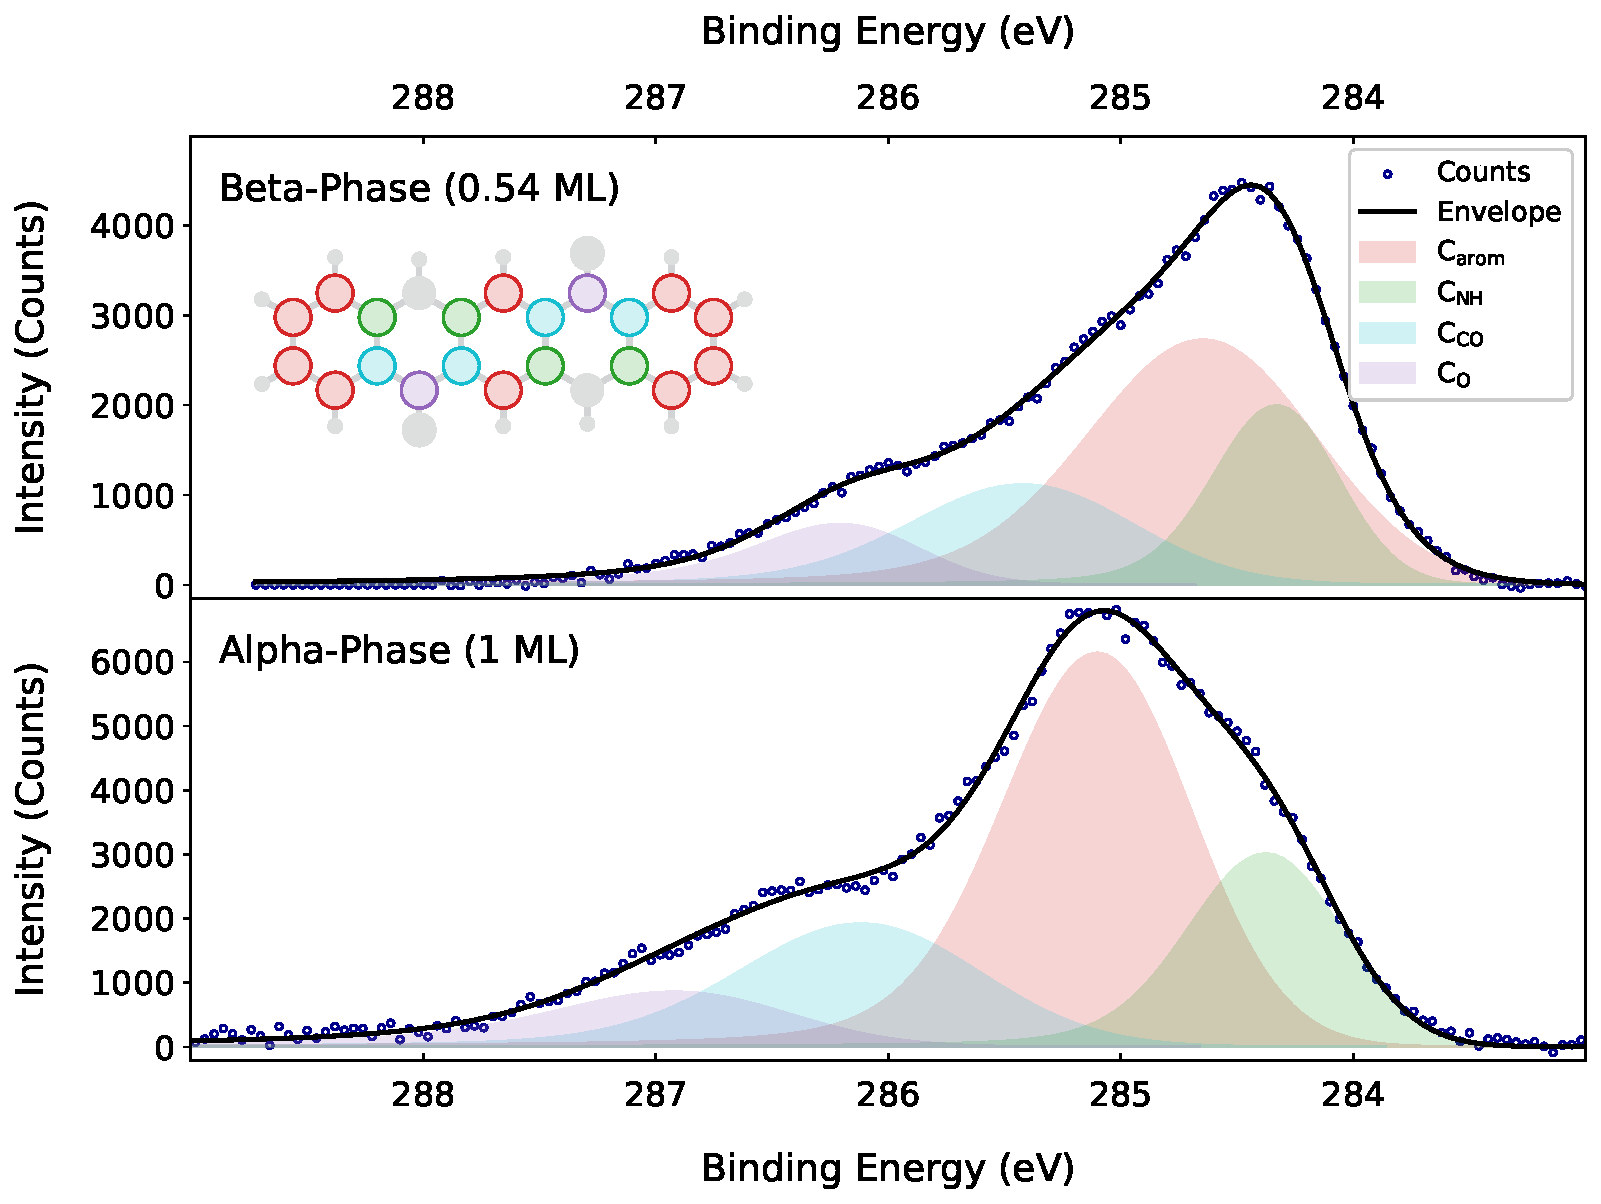
\includegraphics[width=\textwidth]{images/C1s-phase-comparison.pdf}%
                \\ \small{C1s XPS spectra of Quinacridone on Ag(100)}
            \end{center}
        \end{column}
        \begin{column}{0.5\textwidth}
            \begin{center}
                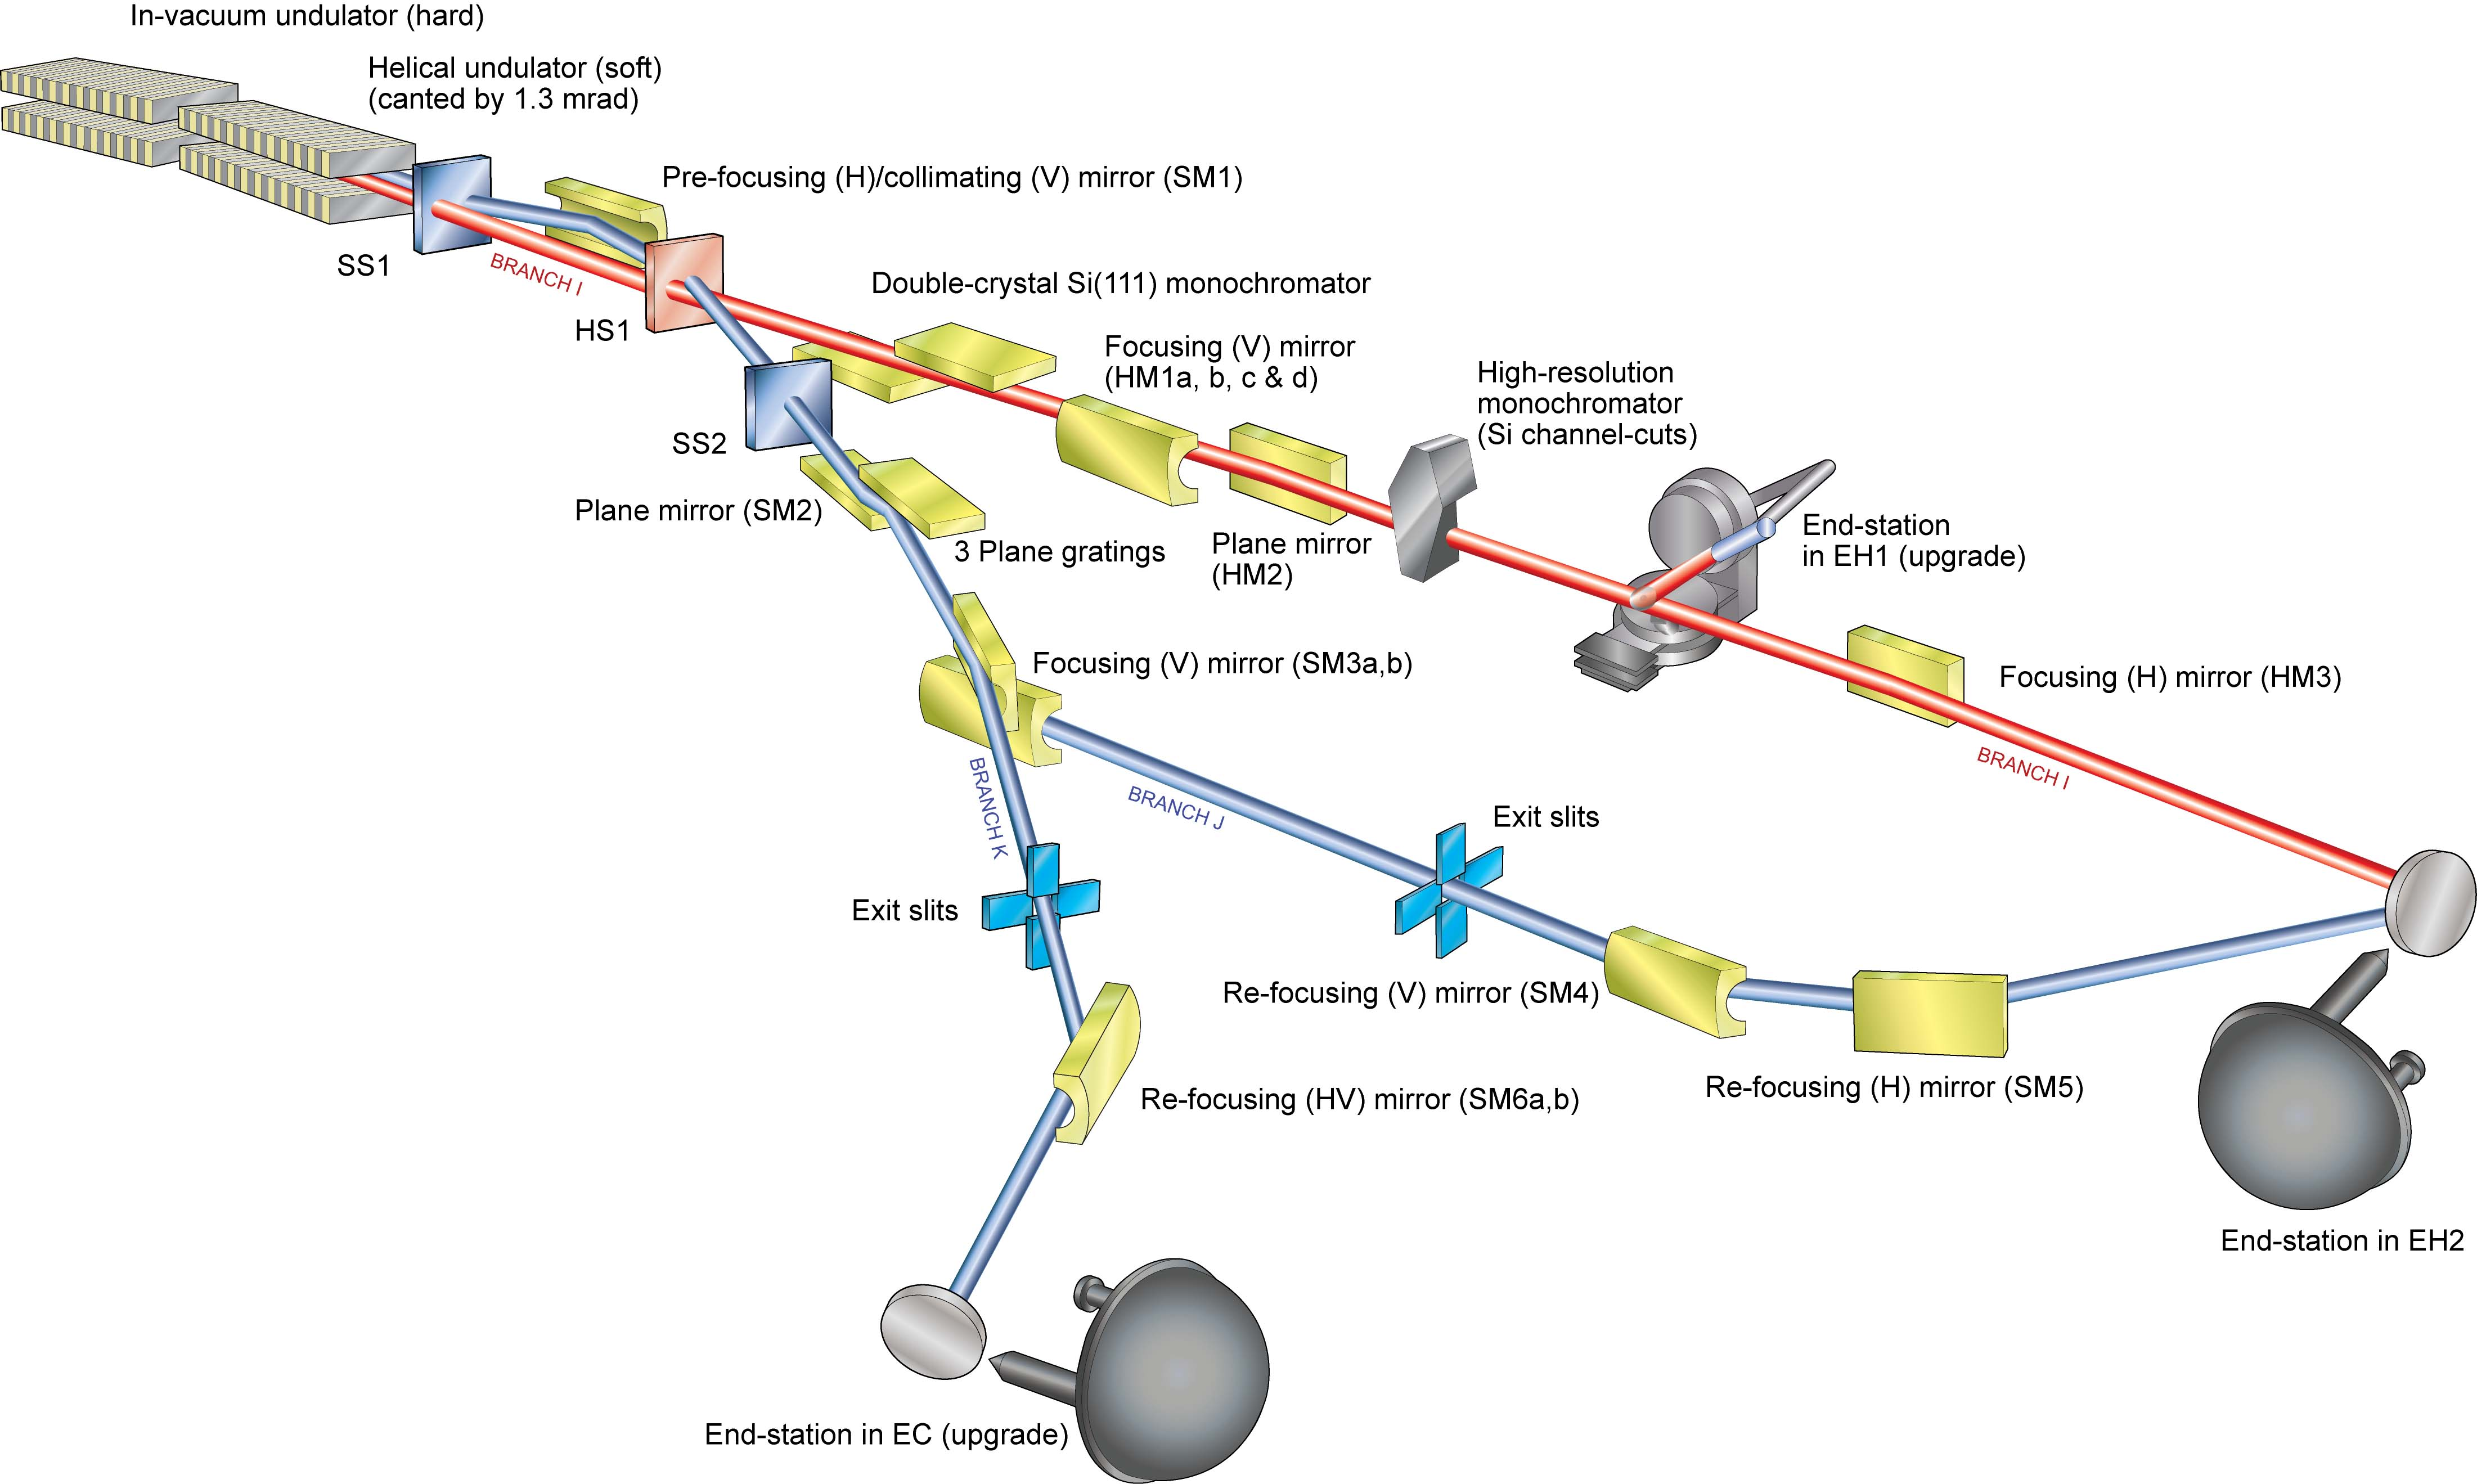
\includegraphics[width=\textwidth]{images/I09.jpg}%
                \\ \small{Diamond Light Source, UK}
            \end{center}
        \end{column}
    \end{columns}
\end{frame}

\begin{frame}{Results of Master Studies}

    \begin{columns}[c]
        \begin{column}{0.5\textwidth}
            \begin{center}
                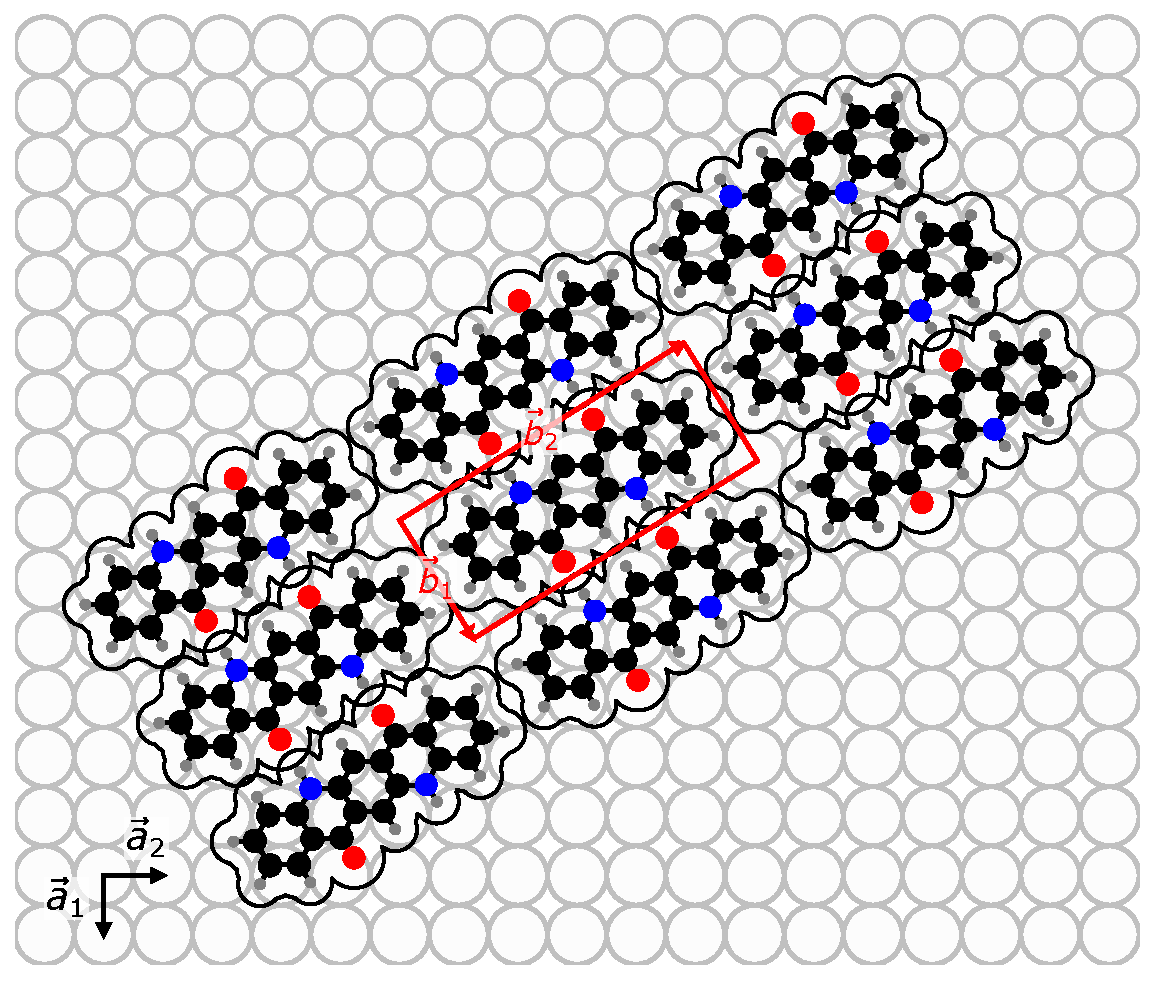
\includegraphics[width=0.75\textwidth]{images/QA-alpha-Ag(100).pdf}%
                \\ \small{$\alpha$-phase of Quinacridone on Ag(100).}
            \end{center}
        \end{column}
        \begin{column}{0.5\textwidth}
            \begin{center}
                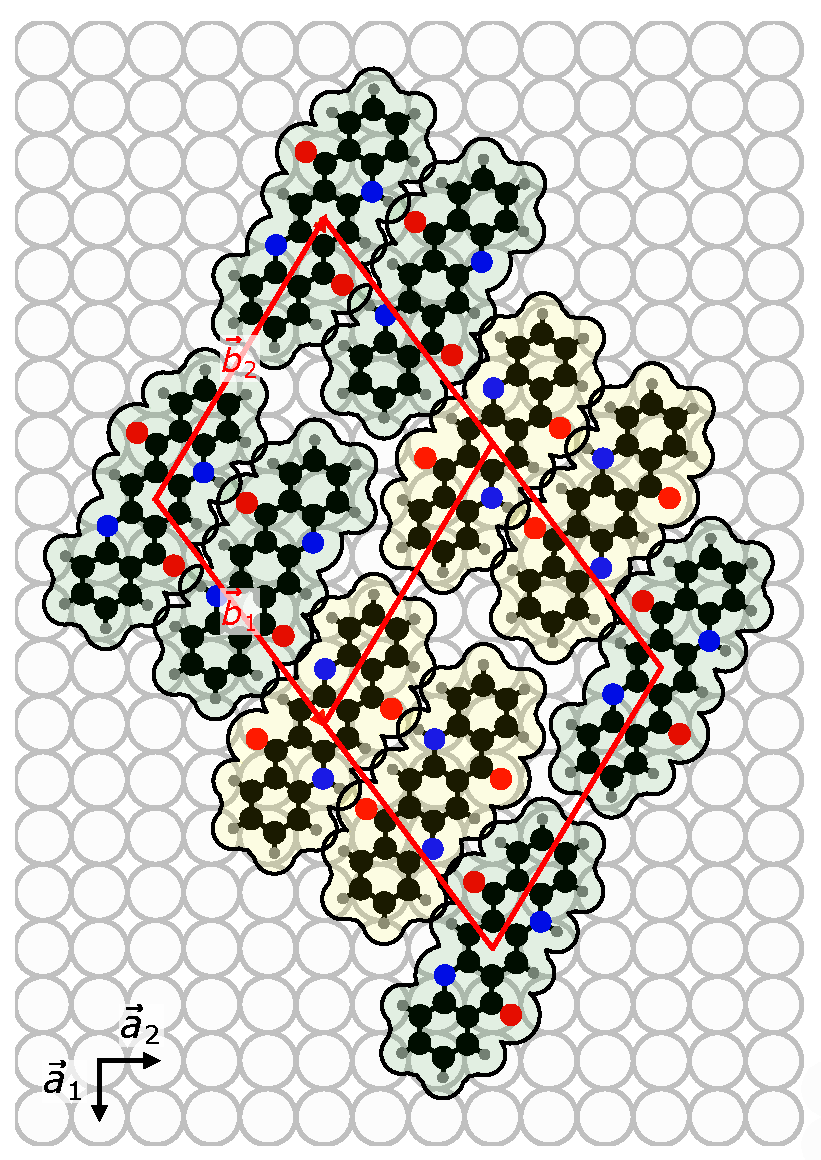
\includegraphics[width=0.6\textwidth]{images/QA-beta-Ag(100)-Version1.pdf}%
                \\ \small{$\beta$-phase of Quinacridone on Ag(100).}
            \end{center}
        \end{column}
    \end{columns}
\end{frame}

% Questions slide
\begin{frame}[c]
    \begin{center}
            \begin{center}
        \setbeamercolor{mybox}{bg=darkbordeaux, fg=white}
        \begin{beamercolorbox}[wd=\textwidth, sep=0.2em, center, rounded=true]{mybox}
            \Huge{Thank You for Your Attention!}
        \end{beamercolorbox}
    \end{center}
        
        \vspace{1em}

        \vspace{2em}

        {\color{darkbordeaux}
            \normalsize
            \faUser\ Lucas Hirschfeld\\
            \faEnvelope\ hirschfeld@pc.uni-bonn.de\\
            \faPhone\ +49 178 1480222
        }
    \end{center}
\end{frame}

\end{document}